\chapter{Setup}
\phantomsection
\section{Unpacking and Connecting the MEGA65}
Time to set up your MEGA65 home computer!
The box contains the following:
\begin{itemize}
\setlength\itemsep{-0.75mm}
\item MEGA65 computer
\item Power supply (black box with socket for mains supply)
\item This book, the MEGA65 User's Guide
\end{itemize}

In addition, to be able to use your MEGA65 computer you may need:
\begin{itemize}
	\item A television or computer monitor with a VGA or digital video input, that is capable of displaying an image at 480p or 576p (720x480 or 720x576 pixel resolution at 50Hz or 60Hz)
\item A VGA video cable, or;
\item A digital video cable
\end{itemize}

These items are not included with the MEGA65.

You may also like to use the following to get the most out of your MEGA65:
\begin{itemize}
\item 3.5mm mini-jack audio cable and suitable speakers or hi-fi system, so that you can enjoy the sound capabilities of your MEGA65.
\item RJ45 Ethernet cable (regular network cable) and a network router or switch. This allows the usage of the high-speed networking capabilities of your MEGA65.
\end{itemize}

\section{Rear Connections}
\index{Display!Connecting}

\includegraphics[width=\linewidth]{images/illustrations/mega65-rear.pdf}
\index{Disk Drives!Connecting}
\begin{center}
\setlength{\def\arraystretch{1.5}\tabcolsep}{6pt}
\begin{longtable}{ c | l}
	1	& 	3.5mm Audio Mini-Jack \\
	2	& 	External microSD Card Slot\\
	3	& 	Network LAN Port \\
	4	& 	Digital Video Connector \\
	5	& 	VGA Video Connector \\
	6	& 	IEC Serial Bus Connector for Disk Drives and Printers \\
	7	& 	Cartridge Expansion Port \\
	8	& 	Power Supply Socket \\
\end{longtable}
\end{center}

%\newpage
\vspace{-1cm}

\section{Side Connections}

\includegraphics[width=\linewidth]{images/illustrations/mega65-side.pdf}

\begin{center}
\setlength{\def\arraystretch{1.5}\tabcolsep}{6pt}
\begin{longtable}{ c | l}
	1	& 	Power Switch \\
	2	& 	Controller Port 2 \\
	3	& 	Controller Port 1 \\
	4	& 	Reset Button \\
\end{longtable}
\end{center}
Various peripherals can be connected to Controller Ports 1 and 2 such as
joysticks, paddles or mouses.

\newpage

\section{MEGA65 Screen and Peripherals}

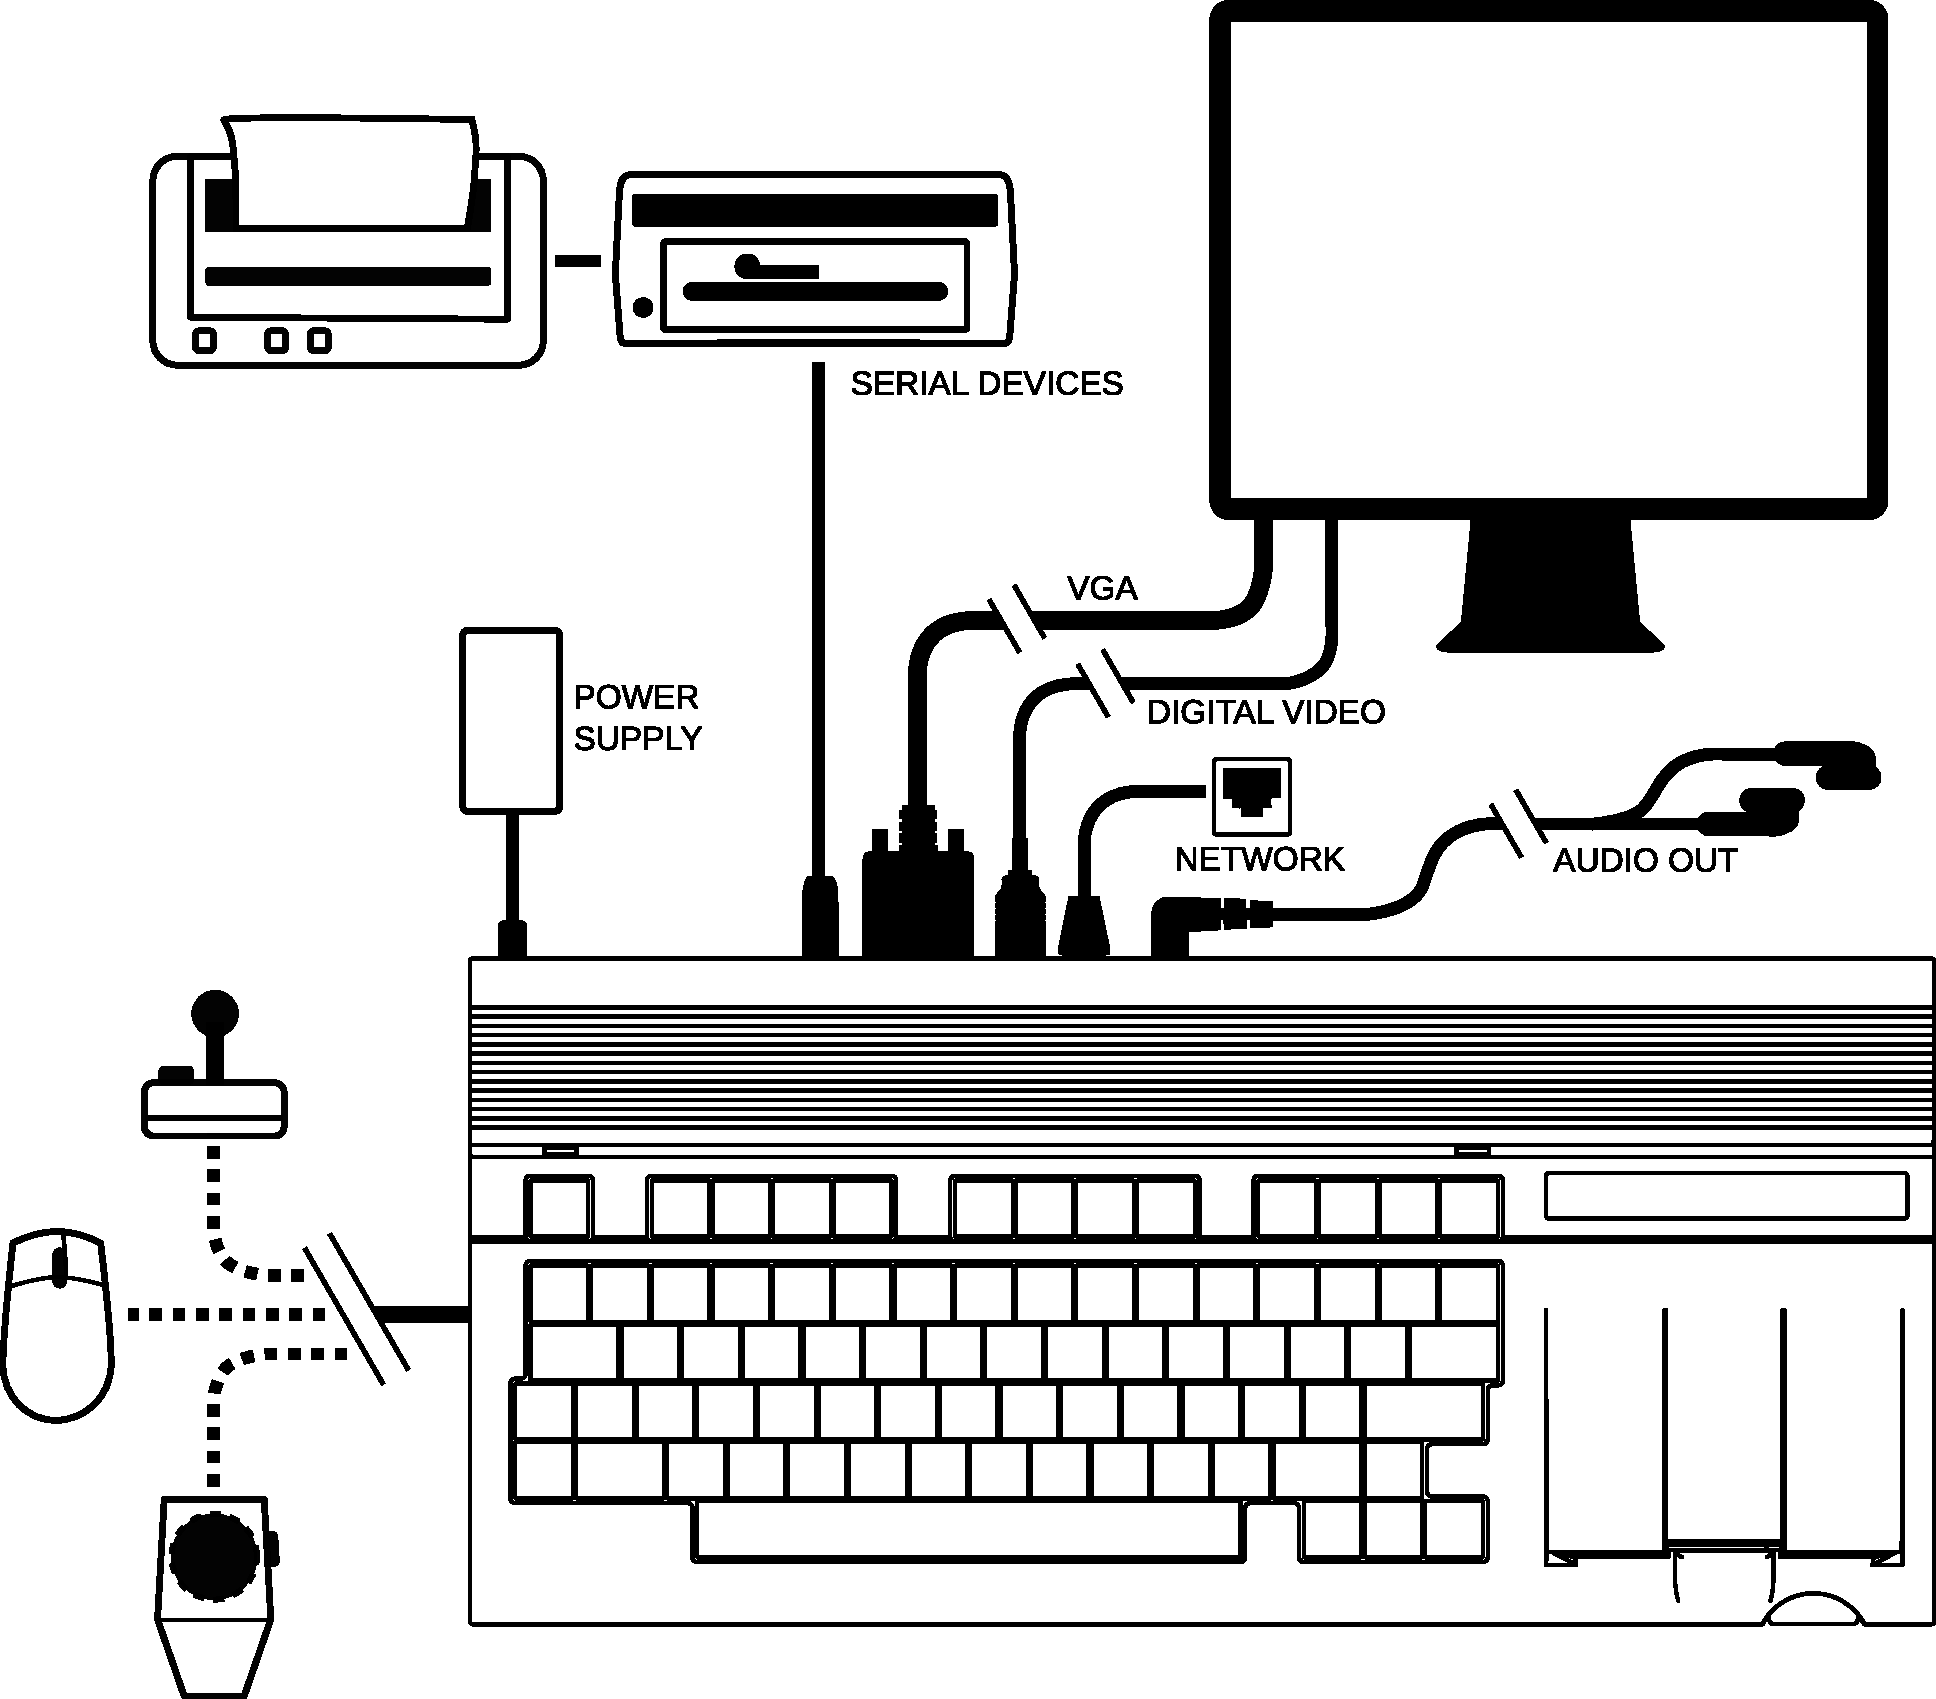
\includegraphics[width=\linewidth]{images/illustrations/mega65-top.pdf}


\begin{enumerate}
	\item Connect the power supply to the power supply socket of the MEGA65.
	\item If you have a VGA monitor and a VGA cable, connect one end to the VGA port of the MEGA65 and the other end into your VGA monitor.
	\item If you have a TV or monitor with a compatible Digital Video connector, connect one end of your cable to the Digital Video port of the MEGA65, and the other into the Digital Video port of your monitor. If you own a monitor with a DVI socket, you can use a Digital Video to DVI adapter.
\end{enumerate}

\newpage
\section{Optional Connections}
\index{Connections!IEC}
\index{SD Cards!Locations}
\begin{enumerate}
	\item The MEGA65 includes an internal 3.5" floppy disk drive. You can also connect older Commodore{\textregistered} IEC serial floppy drives to the MEGA65, such as the Commodore 1541, 1571 or 1581. To use these drives, connect one end of an IEC cable to the Commodore floppy disk drive and the other end to the Disk Drive socket of the MEGA65. You can also connect SD2IEC devices and Pi1541's. It is also possible to daisy-chain additional floppy disk drives or Commodore compatible printers.
	\item You can connect your MEGA65 to an Ethernet network using a standard Ethernet cable.
	\item For enjoying audio from your MEGA65, you can connect a 3.5mm stereo mini-jack cable to an audio amplifier or speaker system. If your system has RCA connectors you will need a 3.5mm mini-jack to twin RCA adapter cable. The MEGA65 also has a built-in amplifier to allow the use of headphones.
	\item A microSD card (either SDHC or SDXC) can be inserted into the external microSD card slot at the rear of the MEGA65.
    \item Underneath the MEGA65, you will find an opening/trapdoor that provides access to the internal SD card slot, and also two PMOD connecters that allow for future possible hardware expansions such as Tape adapters, Userport interfaces, extra memory, or even real SIDs.
\end{enumerate}

\index{Real-Time Clock!Replacing the Battery}
\subsection{Replacing the Real-Time Clock Battery}
The MEGA65 includes a Real-Time Clock, which is used to display the time and date on the startup screen, and to add
timestamps to files that the MEGA65 writes to your SD cards. This clock utilises a CR1220 coin-cell battery to keep
time when the MEGA65 isn't switched on, and unfortunately it doesn't ship with one (this is to minimise the chance
of any international shipping related issues).

To change the battery, you will need to open the case, exposing the motherboard. The case is held together with three
screws, all of which are along the bottom of the front side of the case. Once the three screws have been removed,
{\bf carefully} take the top half of the case off, and note the orientation of the keyboard connector, before
disconnecting it.

The battery is located between the controller ports and the keyboard connector:

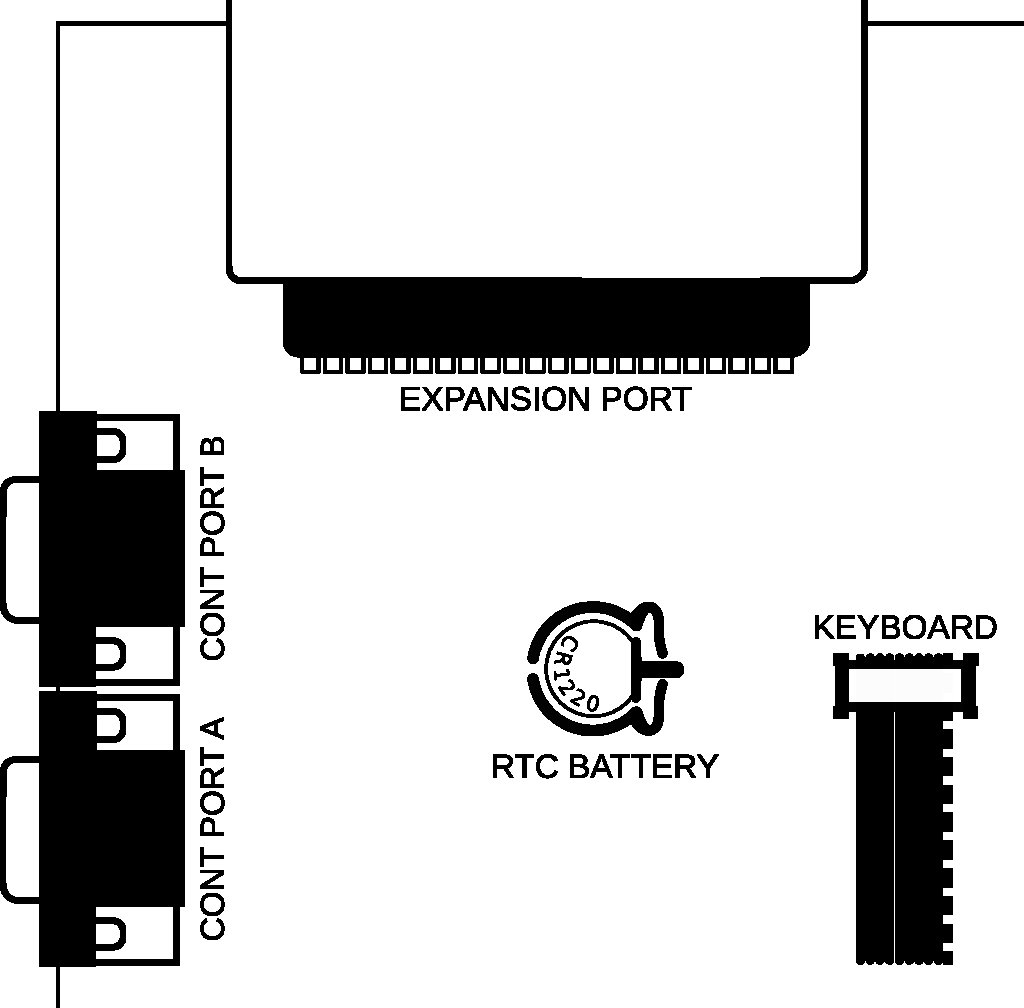
\includegraphics[width=10cm]{images/illustrations/rtc-battery-location.pdf}

If you are removing an existing battery, push the battery release lever on the bottom (flat-sided) side of the
battery socket \textit{away} from the battery to remove it. Next, insert the new battery with the side labelled
{\bf + facing up}, and press it into place.

Once you have re-assembled your MEGA65, you can set the time in the Configure menu. You can read more about setting
the time on page \pageref{configuring-chipset}.




\section{Operation}

\subsection{Using the MEGA65}

\begin{enumerate}
	\item Switch on the MEGA65 by using the switch on the left-hand side. \newline \newline
    \underline{Note}: On first power up, you will see an On-Boarding screen. See page \pageref{onboarding} for more details. \newline
    \begin{center}%
      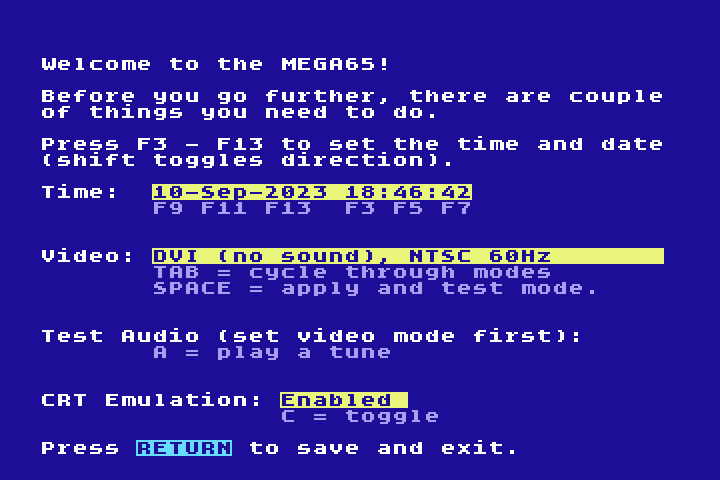
\includegraphics[trim= 10mm 140mm 10mm 10mm,clip,width=0.9\linewidth]{images/img011_final_boot_01.png}%
    \end{center}
	\item After a moment, the following will be displayed on your TV or monitor:
\end{enumerate}

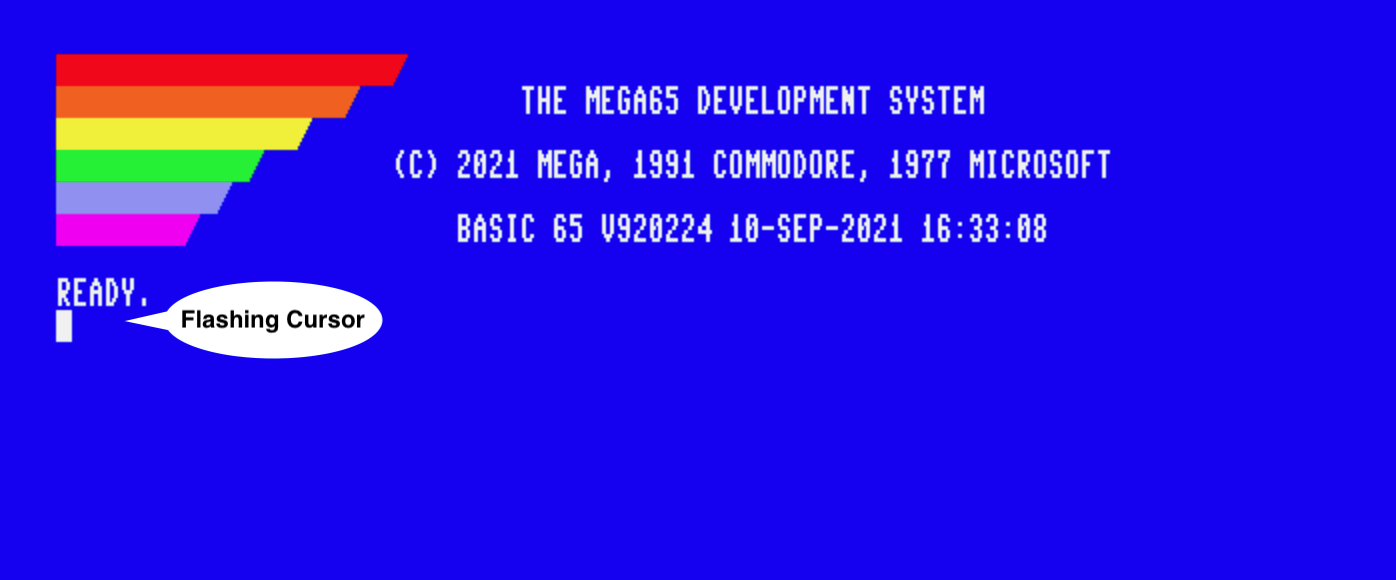
\includegraphics[width=\linewidth]{images/introduction-screen/switched-on.png}

\subsection{The Cursor}

The flashing square underneath the \screentext{READY} prompt is called the cursor. The cursor indicates that the computer is ready to accept input. Pressing keys on the keyboard will print their respective characters onto the screen. The characters will be printed at the current cursor position, and the cursor will advance to the next position after every key press.

Here you can type commands, that can do things such as loading a program. You can also start entering program code!
